\lstset{style=mystyle}

\section{Querying the collection}

\subsection{Find documents whose tags contain the word "mongodb"}

\begin{lstlisting}
    db.post.find({tags: {$in: ["mongodb"]}})
\end{lstlisting}


\subsection{Find documents whose descriptions contain the word "NoSQL" (using text search)}

\begin{lstlisting}
    db.post.createIndex({description: "text"})
    db.post.find({$text: {$search: "NoSQL"}})
\end{lstlisting}

\subsection{Find documents whose titles or descriptions contain the word "NoSQL"}

\begin{lstlisting}
    db.post.createIndex({description: "text", title: "text"})
    db.post.find({$text: {$search: "NoSQL"}})
\end{lstlisting}

\subsection{Find documents having more than 50 likes}

\begin{lstlisting}
    db.post.find({likes: {$gt: 50}})
\end{lstlisting}

\subsection{Find the average likes number of documents with tags containing the word "mongo" in the collection}

\begin{lstlisting}
    db.post.aggregate([{
        $match: {
            tags: {
                $in: ["mongo"]
            }
        },
        $group: {
            _id: null,
            avg: {$avg: "$likes"}
        }
    }])
\end{lstlisting}

\clearpage

\section{Replication}

\subsection{See the status of rs0 and add data to the primary instance, check if the data appears on the secondary instance.}

\begin{figure}[!h]
    \begin{center}
        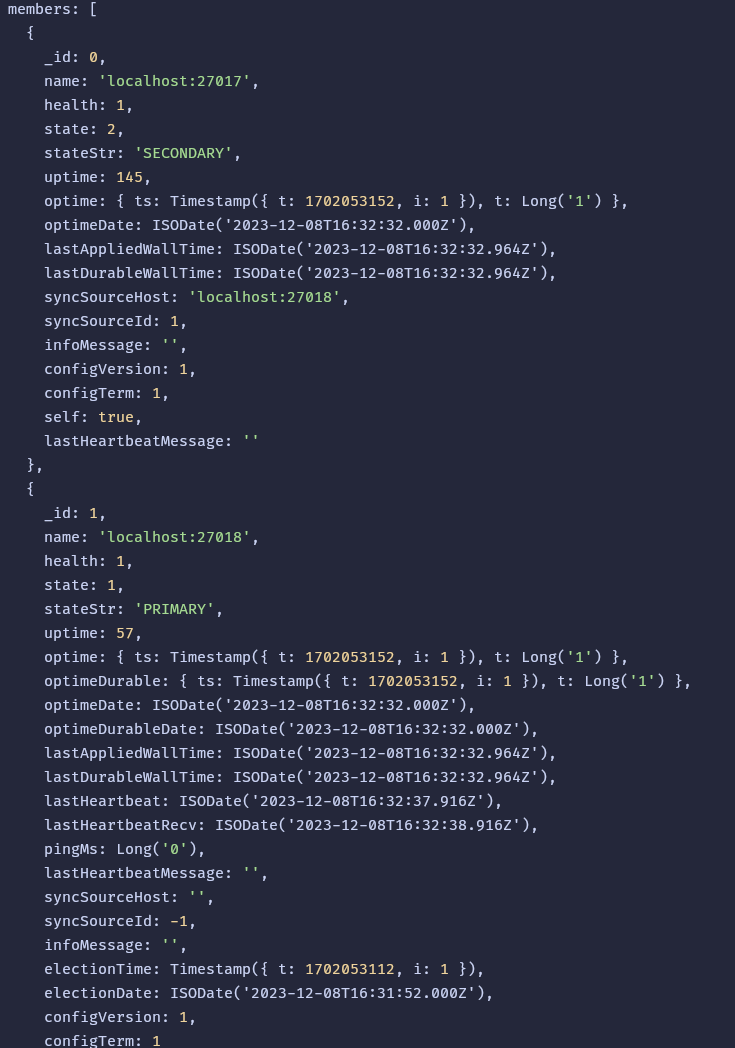
\includegraphics[width=10cm]{rs0_status}
        \caption{Status of rs0 after initializing with two instances}
    \end{center}
\end{figure}

\begin{figure}[!h]
    \begin{center}
        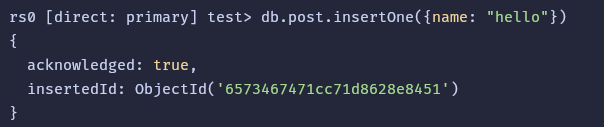
\includegraphics[width=10cm]{rs0_primary_insert}
        \caption{Insertion of data in primary instance}
    \end{center}
\end{figure}

\begin{figure}[!h]
    \begin{center}
        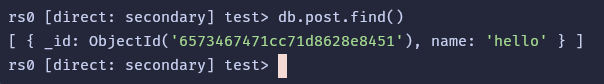
\includegraphics[width=10cm]{rs0_secondary_find}
        \caption{Querying data in secondary instance}
    \end{center}
\end{figure}

\subsection{Stop the primary instance, check the status of rs0 again, and see which secondary instance becomes the primary}

\begin{figure}[!h]
    \begin{center}
        \resizebox{\textwidth}{!}{
            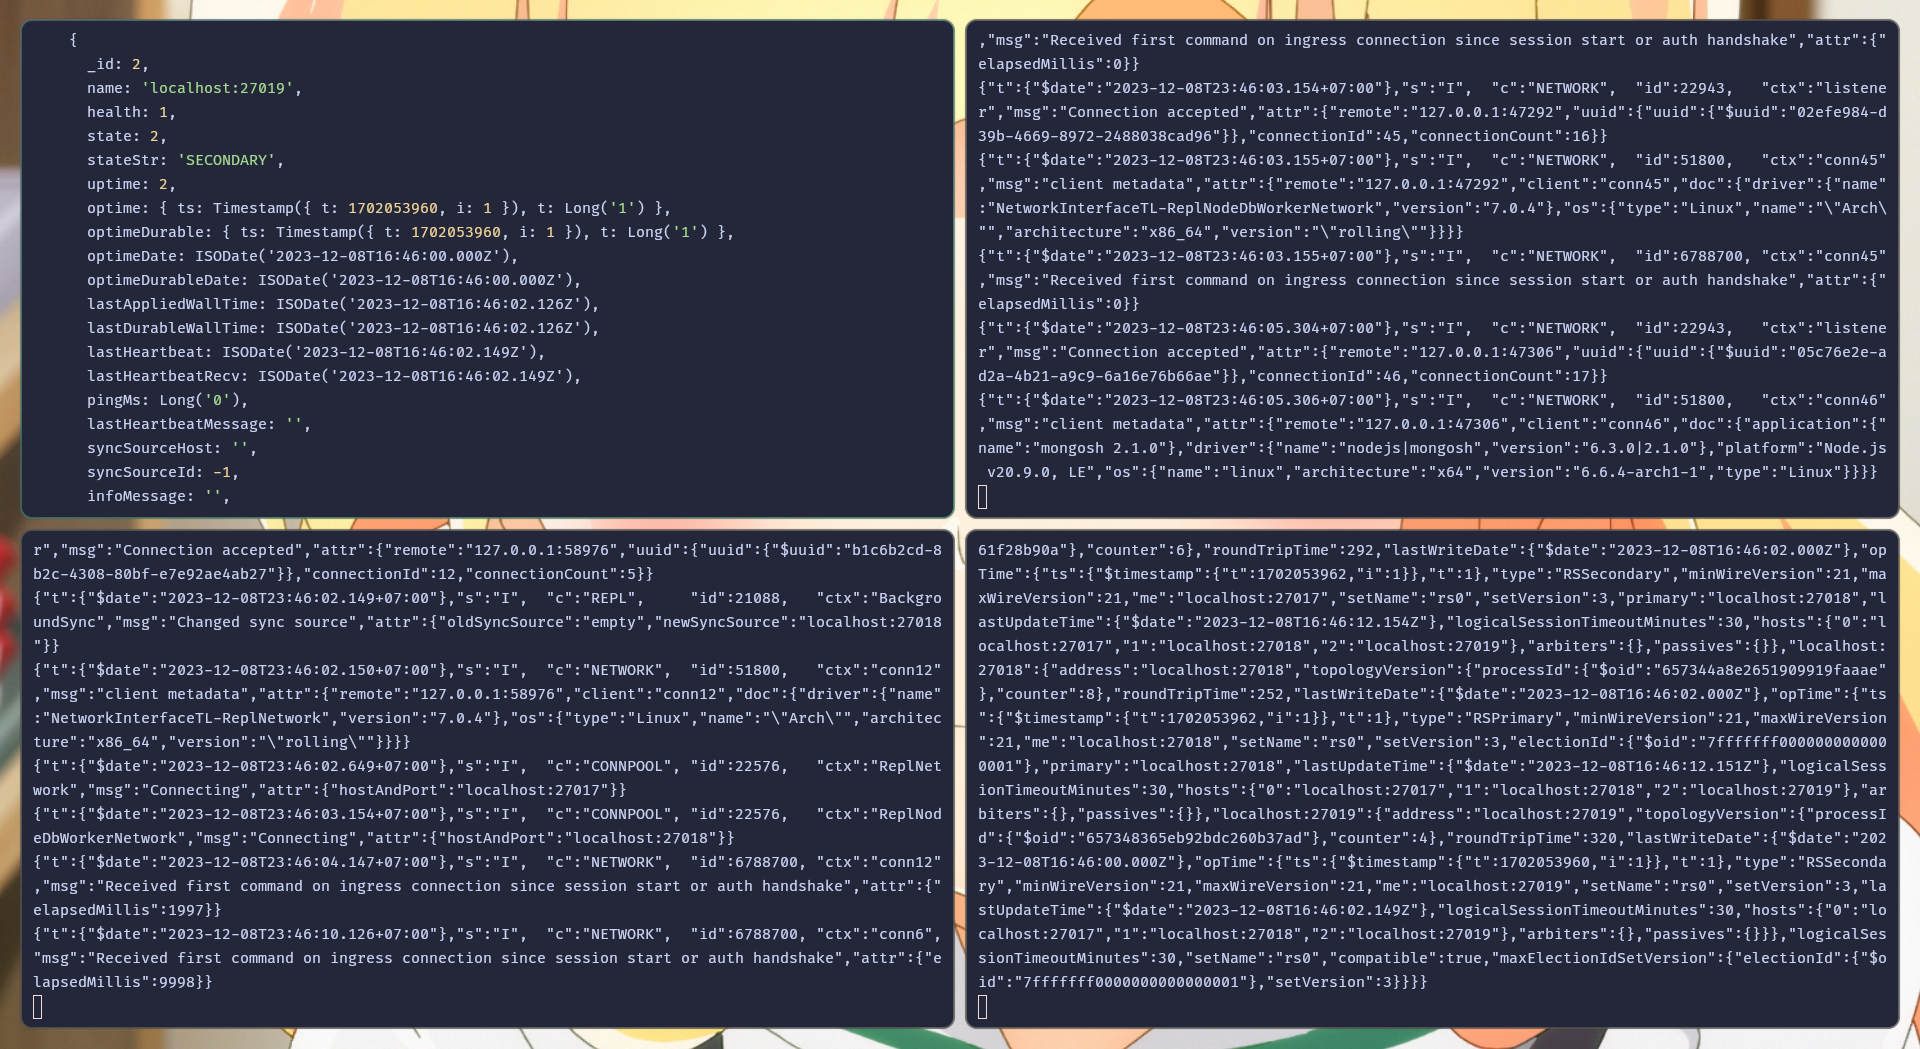
\includegraphics[width=10cm]{rs0_add_third_instance}
        }
        \caption{MongoDB running with three instances}
    \end{center}
\end{figure}

\begin{figure}[!h]
    \begin{center}
        \resizebox{\textwidth}{!}{
            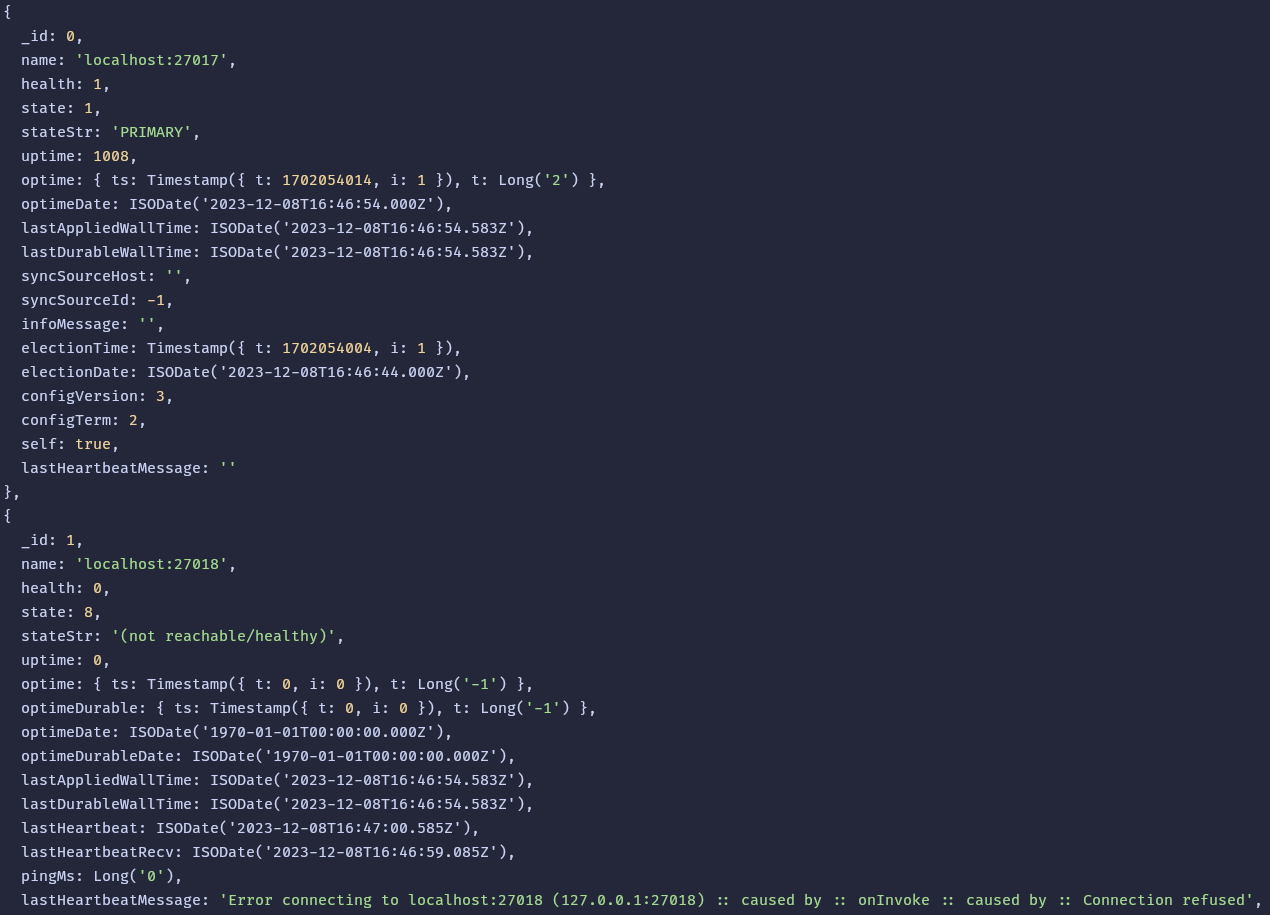
\includegraphics[width=10cm]{rs0_ending_old_primary}
        }
        \caption{Status after ending old primary instance.}
    \end{center}
\end{figure}

As it can be noticed, the instance with the lower ID or the lower port number
will turn into the new primary for the replica set.